%%% Fiktivní kapitola s ukázkami sazby

\chapter{Analýza problému a jeho řešení}

V této kapitole je detailně popsán problém a způsoby jeho navrženého a současného řešení.

\section{Úvod}

Spoje které zajišťují hromadnou dopravu jezdí podle jízdních řádů, které definují jejich trasu. Trasa se udává sekvencí projíždících zastávek, časy příjezdu a odjezdu do, resp. z těchto zastávek a vzdáleností zastávek od výchozího bodu spoje. Tyto zastávky jsou zpravidla jediné refenční body u kterých je možno zjistit skutečné zpoždění, nebo předjetí (dále uvažováno jako zpoždění se zápornou hodnotou). Dále jsou součástí jízdních řádů také velice detailní nákresy tras každého spoje, formou lomené čáry definovanou posloupností souřadnic, kde každý bod je doplněn o jeho vzdálenost od výchozího bodu spoje.

\bigbreak

Délka trasy mezi dvěma refernčními body nezříka dosahuje i několika desítek kilometrů\footnote{Podle dat pro spoje jedoucí v 20. 2. 2020 je medián vzdálesnotí mezi zastávkama, mezi kterýma projede alesponˇ jeden spoj denně 943 m. Průjezdů mezi zatávkami ve vzdálenosti více než 10 kilometrů je 784, přiřičemž průjezdů mezi zastávkami ve vzdálenosti alesponˇ 2 km je přibližně 15000}. Na těchto úsecích mohou vznikat mimořáné události, které se dají predikovat jen s těží. Nicméně ve většině případů je průběh jízdy ovlivněn pouze obvyklým provozem v dané denní době.

Detailní rozbor počtu průjezdů mezi zastávkami v daných vzdálenostech je vidět na grafu \ref{fig:stop_distances_result}. Kde průjezdem se myslí každý jednotlivý průjezd vozidla mezi danou dvojcí zastávek v daný den. Data jsou platná pro spoje jedoucí v 20. 2. 2020.

\begin{figure}
  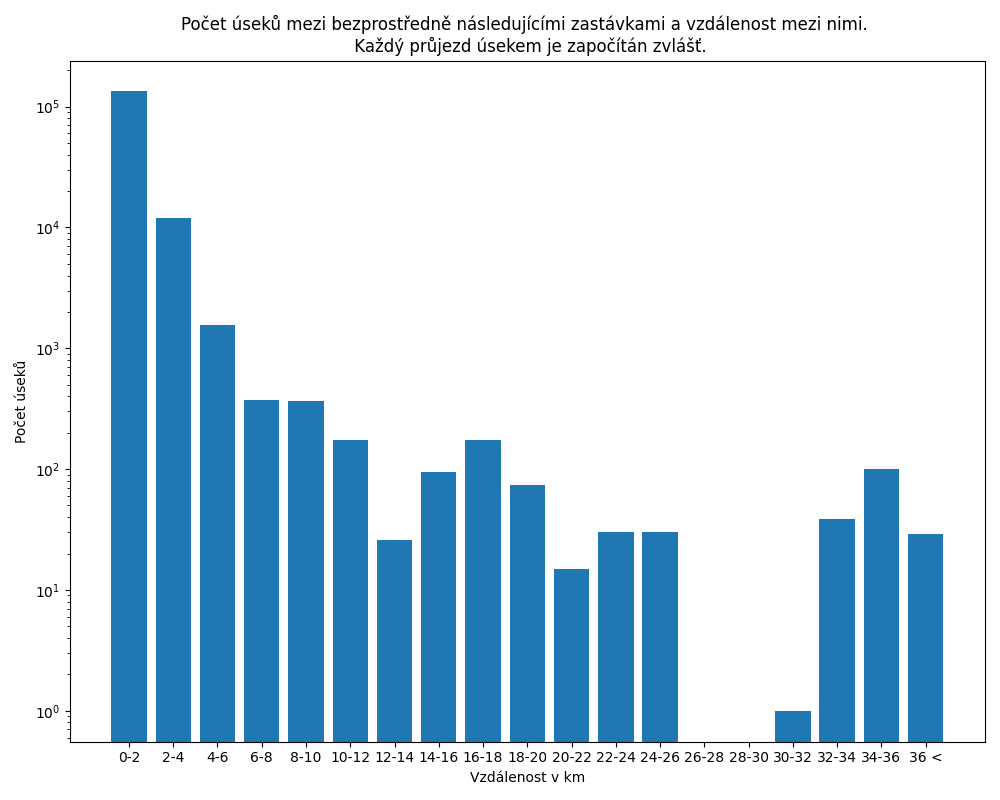
\includegraphics[width=\linewidth]{../img/stop_distances_plot_2020-02-20.png}
  \caption{Graf počtu úseků mezi následujícími zastávkami a vzdálenotí mezi nimi.}
  \label{fig:stop_distances_result}
\end{figure}

\section{Popis problému odhadu zpoždění}

Řešený problém se týká případu, kdy vozidlo projíždí mezi dvěma referenčními body a tato trasa má části, ve kterých vozidlo jede různou rychlostí. Např. vozidlo při vyjíždění z města jede mnohem pomaleji než při jízdě mezi městy. Takových úseků, na kterých se rychlost jízdy liší může být na trase více a nedají se všechny jednoduše detekovat.

\bigbreak

Tato Práce tedy modeluje profily jízd mezi referenčními body. A na základě toho zpřesnit odhad zpoždění. Tento odhad by měl být mnohem přesnější než současné odhady, které odpovídají tomu, že vozidlo jede konstantní rychlostí po celou dobu jízdy. Nebo je takové možné brát jako aktuální zpoždění spoje poslední změřené zpoždění při průjezdu nějak7ch referenčním bodem (zastávkou, nebo např. pro tramvaje se používají návěstidla).

\bigbreak

Přidaná hodnota je tedy v tom, že Práce navrhne takové modely, které nebudou penezalizovat zvyšováním zpožděním za pomalou jízdu v úsecích, které se pomaleji projždějí vždy. A také naopak zvýhodnˇovat snížením zpožděním za rychlou jízdu v úsecích, které se projíždějí rychle. Pokud bychom se tedy podívali na změny zpoždění na trase mezi dvěma referečními body, v ideálním případně by měli být nulové.

\bigbreak

Celé ilustrováno na příkladě.

\bigbreak

Pro řešení toho typu spoždění stačí navrhnout systém na odhat zpoždění v půběhu jízdy mezi referenčními body z historikých dat jízd.

\bigbreak

Tento odhad změny zpoždění na trase mezi dvěma referenčními body je nutné počítat v co nejkratším čase tak, aby cestující byli dobře informování o stavu jejich spoje a mohli tyto informace využít např. při dobíhání spoje. A proto je potřeba zpracovávat data okamžitě po jejich vydání, spočítat odhad zpoždění a vystavit tato data veřejně. Vzhledem k tomu, že tato data velmi rychle zastarávají je nutné provádět tento proces co možná nejrychleji\footnote{Průměrná doba jízdy spoje mezi zastávkami je cca 5 min. Rozložení počtu úseků mezi zastávekami k délce jízdy mezi nimi je závislé a podobné rozložení vůči vzdálenosti ilustrované na grafu\ref{fig:stop_distances_result}.}.

\bigbreak

Pro vyloučení všech pochybností je hodno uvést, že se naše Práce nesnaží předpovědět zpoždění, které spoj může nabrat vzhledem k dosavadnímu průběhu trasy. Tedy např. nijak nezohlednˇuje to, že spoj právě stojí v mimořádné koloně a dalo by se tedy předpokládat, že zpoždění bude rychle růst i v následujících minutách. Ale naopak Práce se snaží odhadnou zpoždění v danném bodě na trase vzhledem k obvyklému profilu jízdy. Tedy např. pokud by výše uvažavaná kolona byla pravidelná Práce ji zohlední ve statistických modelech.

\subsection{Současná řešení}

Takový algoritmus na odhat aktuálního zpoždění mezi dvěma referenčními body již exituje a je zakomponován v systému, ze kterého se čerpají data pro tuto práci. (Detailní popis dat uveden v kapitole ~\ref{chapter:TODO later}.) Nicméně nezohledňuje základní parametry průběhu trasy. Tento algoritmus nahlíží na postup vozidla na trase jako na lineární funkci vůči času. Je ovšem zřejmé, že rychlost vozidel není konstantní, neboli doba jízdy není linárně závislá na ujeté vzdálenosti.

\section{Analýza požadavků na uživatelskou aplikaci}

Součástí práce je i vizualizace spočítaných dat. Jinými slovy nástroj umožňující přístup uživatelů ke spočítaným datům.

\subsubsection{Funkční požadavky}

\begin{itemize}
	\item Aplikace vykreslí interaktivní mapu Prahy a širšího okolí, kterou bude možné posouvat či zoomovat. V této mapě budou zobrazeny jednotlivé vozidla na aktuálních pozicích a budou se automaticky posouvat po mapě, tak jak se pohybují ve skutečnosti.

	\item Po kliknutí na vozidlo se zobrazí jeho celá trasa včetně zastávek a jeho dopočítaného zpoždění.

	\item Po kliknutí na zastávku se zobrazí seznam spojů, které budou projíždět vybranou zastávkou a jejich trasy se vykreslí do mapy.

	\item Celá aplikace bude postavena na principu server -- client. Tedy serverová strana se postará o přístup k otevřeným datům o vozidlech a jejich uložení a také obsluhu požadavků klienta. Klientská část bude webová stránka poskytující služby popsané výše. Měla by být schopná zobrazit řádově tisíce vozidel.
\end{itemize}

\subsubsection{Nefunkční požadavky}

\begin{itemize}
	\item Serverová část bude napsaná v jazyce Python 3.

	\item Webová část bude napsaná pomocí jazyků pro webové technologie, převážně v JavaScriptu.

	\item Pro vykleslení mapy bude využita služba Mapbox.

	\item Ukládání dat na serverové straně bude řešeno MySQL databází.

	\item Pro algoritmus odhadu zpoždění na zákldě historických dat budou využity různé knihovny pro jazyk Python 3. Zejména pak scikit-learn a alphashape.

\end{itemize}

\subsubsection{Proces běhu aplikace}

Jak je již zmíněno aplikace bude využívat historická data, tedy bude nutné nechat aplikaci tato data nějakou dobu sbírat. Pro efektivní odhady by bylo vhodné mít uložené historické polohy vozidel alespoň z uplynulých několika týdnů.

\bigbreak

Avšak již v průběhu sběru dat může aplikace poskytovat základní službu a to vizualizování vozidel v mapě.

\subsection{Poskytovatelé mapových podkladů}

K takovému účelu nejlépe poslouží vykreslení aktuálních poloh vozidel do mapy, kde se po vyžádání uživatelem tyto data zobrazí.

\bigbreak

Za účelem vytvoření dostatečně přívětivé uživatelské aplikace je nezbytné využít některého z poskytovatelů mapových podkladů a zanést do něj získané informace.

\bigbreak

Jedním z těchto poskytovatelů je společnost Google, která má propracované mapové podklady a prostřednictvím služby Google Maps poskytuje pro tuto práci požadovanou službu. Další platformou je Mapbox, který poskytuje velmi podobné služby jako Google Maps. Nicméně narozdíl od Googlu využívá jako mapový podklad \gls{osm} {otevřená geografické data}. Protože smyslem práce je v co největší míře využít otevřená data je žádoucí využít právě Mapbox.

\bigbreak

TODO dokumentace mapbox, zeptat se jestli je to vubec nutne rozebirat

\subsection{Současná řešení}

Vizualizaci vozidel \gls{vhd} do mapy již nabízí několik portálů. Všechny jsou však poměrně strohé.

\subsubsection{Golemio}

Takovou mapu zobrazuje i samotný provozavatel datové platformy. Nicméně nejsou zde vidět ani čísla linek zobrazených autobusů, natož pak nějaké další informace.

\begin{figure}
  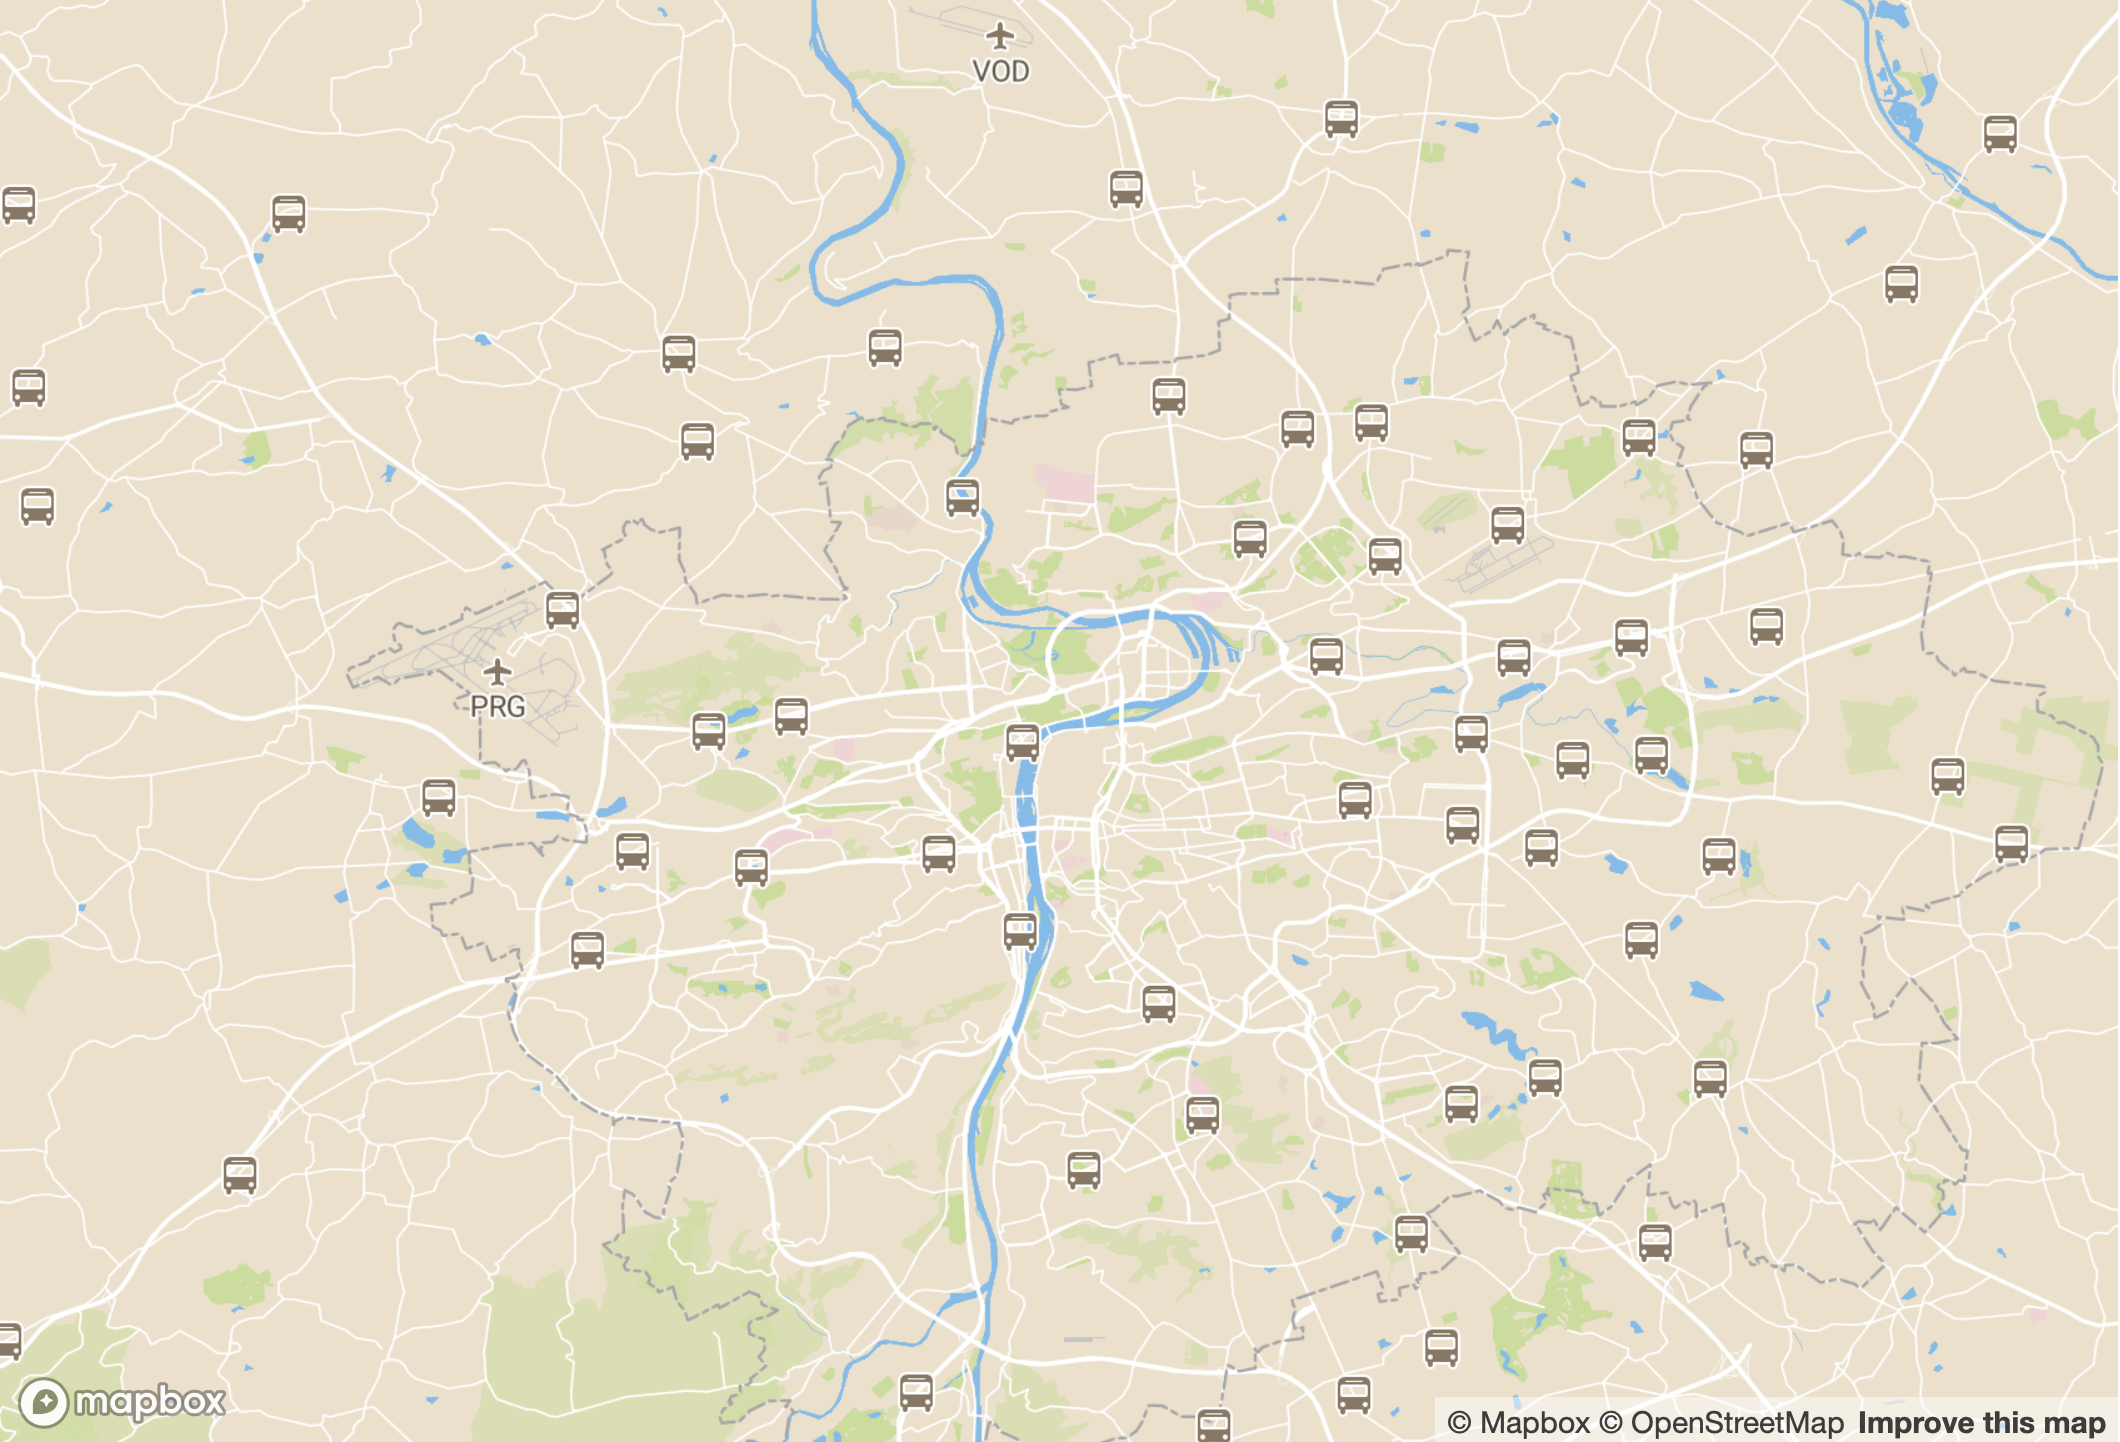
\includegraphics[width=\linewidth]{../img/golemio_mapa.png}
  \caption{Mapa z golemio.cz.}
  \label{fig:golemio_result}
\end{figure}

\subsubsection{Tram-bus}

Dalším poskytovatelem je portál tram-bus, který si vede o něco lépe. Ukazuje směr jízdy vozidel, čísla linek a po kliknutí informace o zpoždění a nejbližší zastávky. Pozn.: na mapě již jsou vidět spoje \gls{dpp}, protože v době psaní této práce již byly data veřejné.

\begin{figure}
  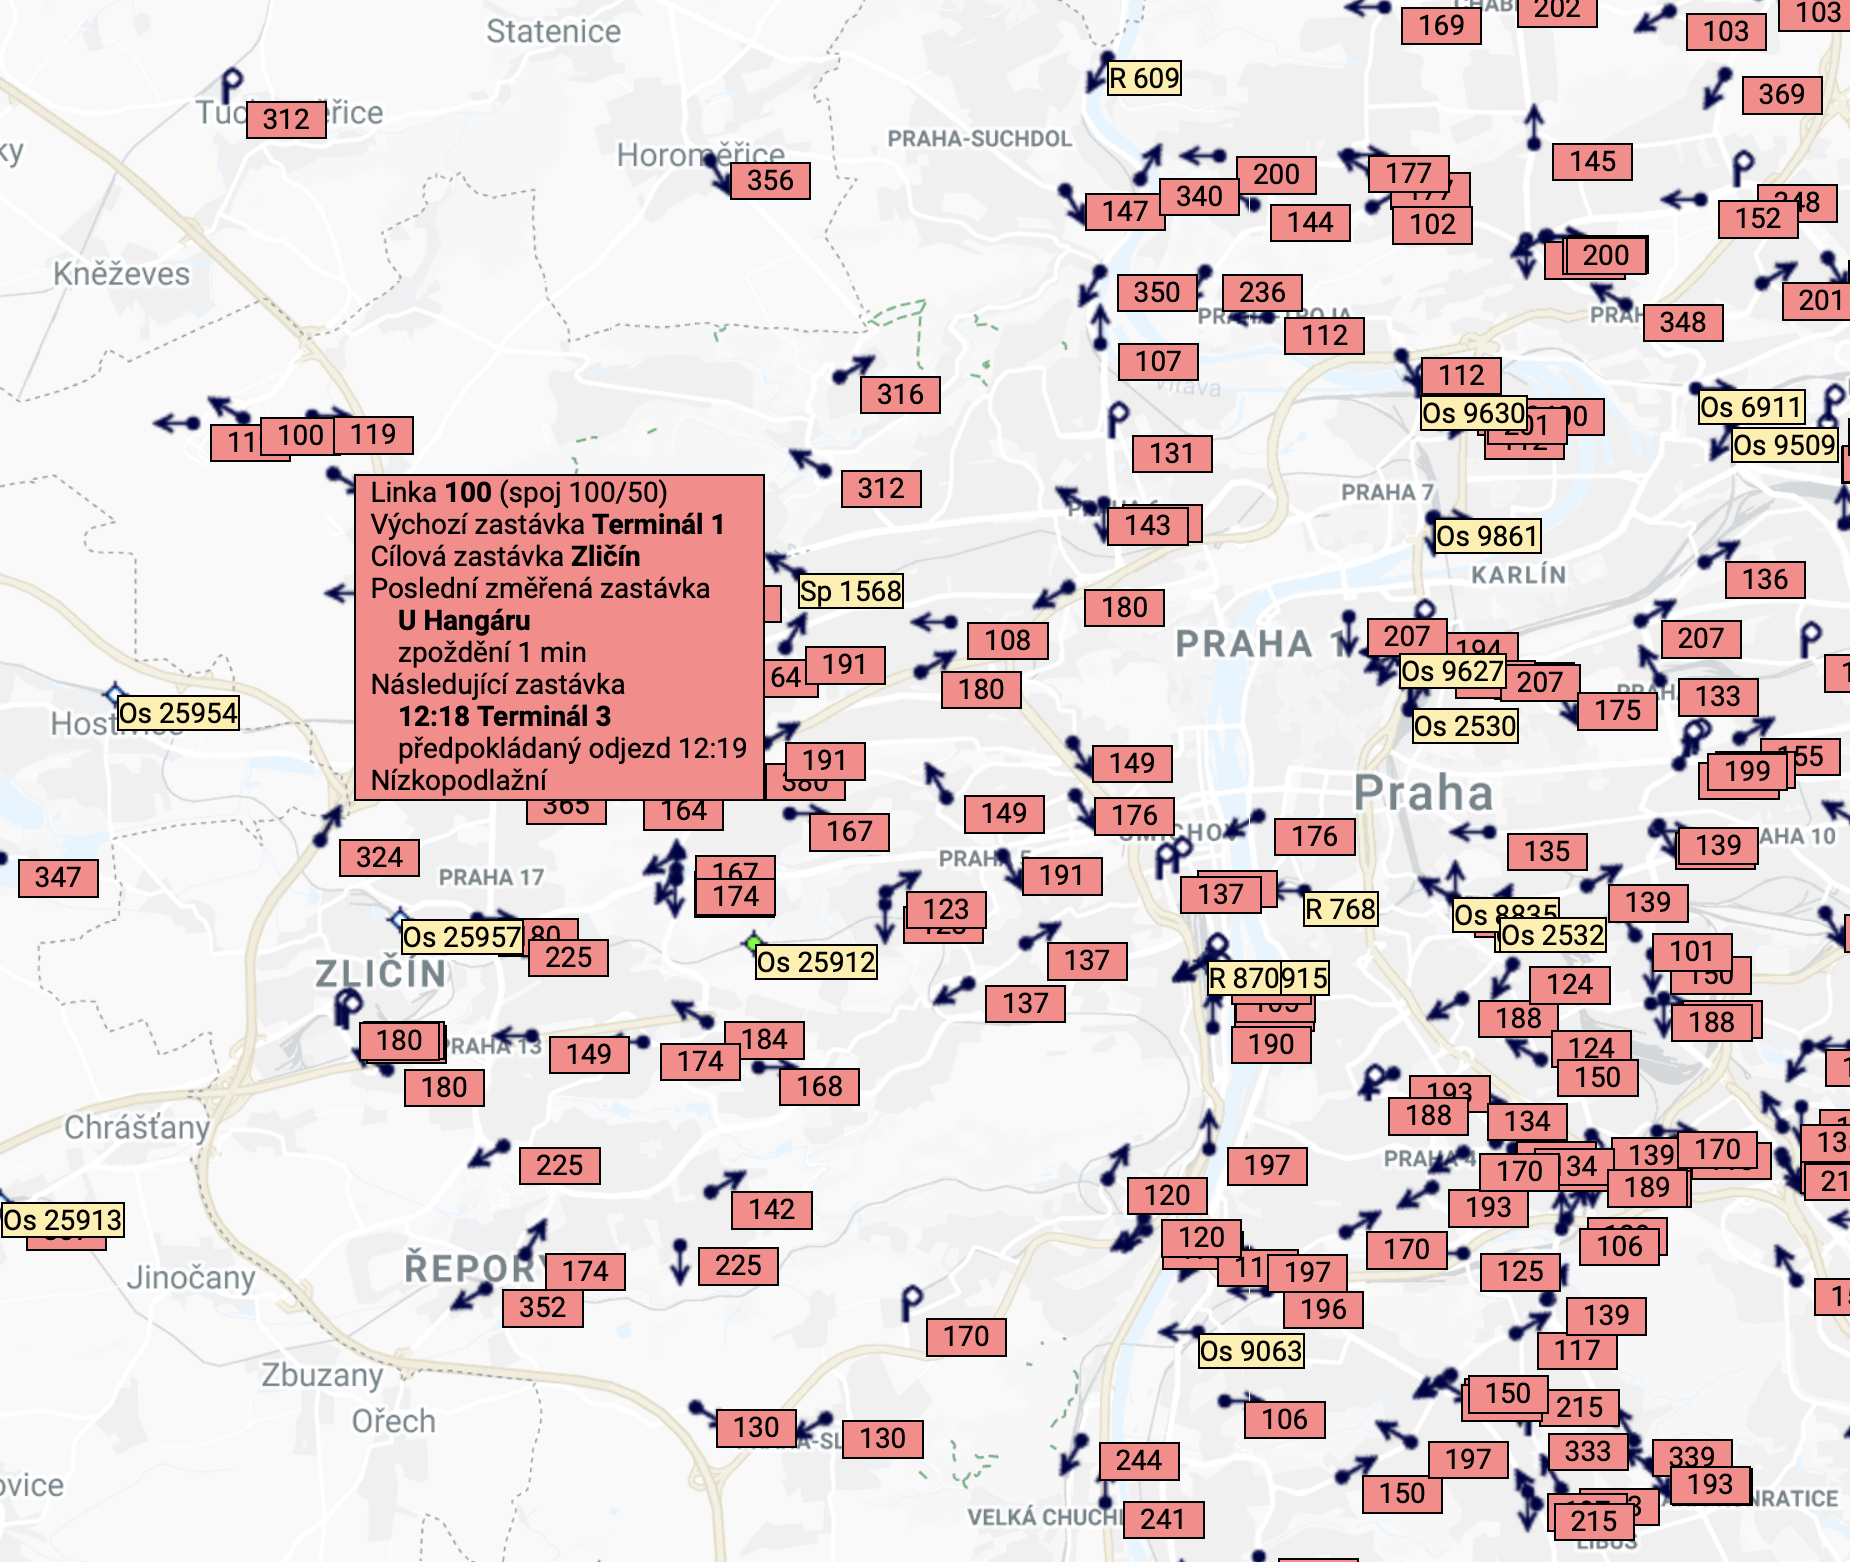
\includegraphics[width=\linewidth]{../img/tram-bus_mapa.png}
  \caption{Mapa z www.tram-bus.cz.}
  \label{fig:tram-bus_result}
\end{figure}

\subsubsection{\gls{idsjmk}}

Mimo Prahu je velice pěkně udělaná aplikace pro zobrazení vozidel \gls{idsjmk} (Integrovaný dopravní systém Jihomoravského kraje). Ten ihned po načtení stránky zobrazuje všechny dobravní prostředky, tedy tramvaje, autobusy a vlaky vše s čísly linek. Dále pak umožňuje po kliknutí na vybraný spoj zobrazit více informací včetně jízdního řádu.

\bigbreak

Tato aplikace je po vizuální i funkční stránce dobrou inspirací pro tvorbu aplikace v této práci.

\begin{figure}
  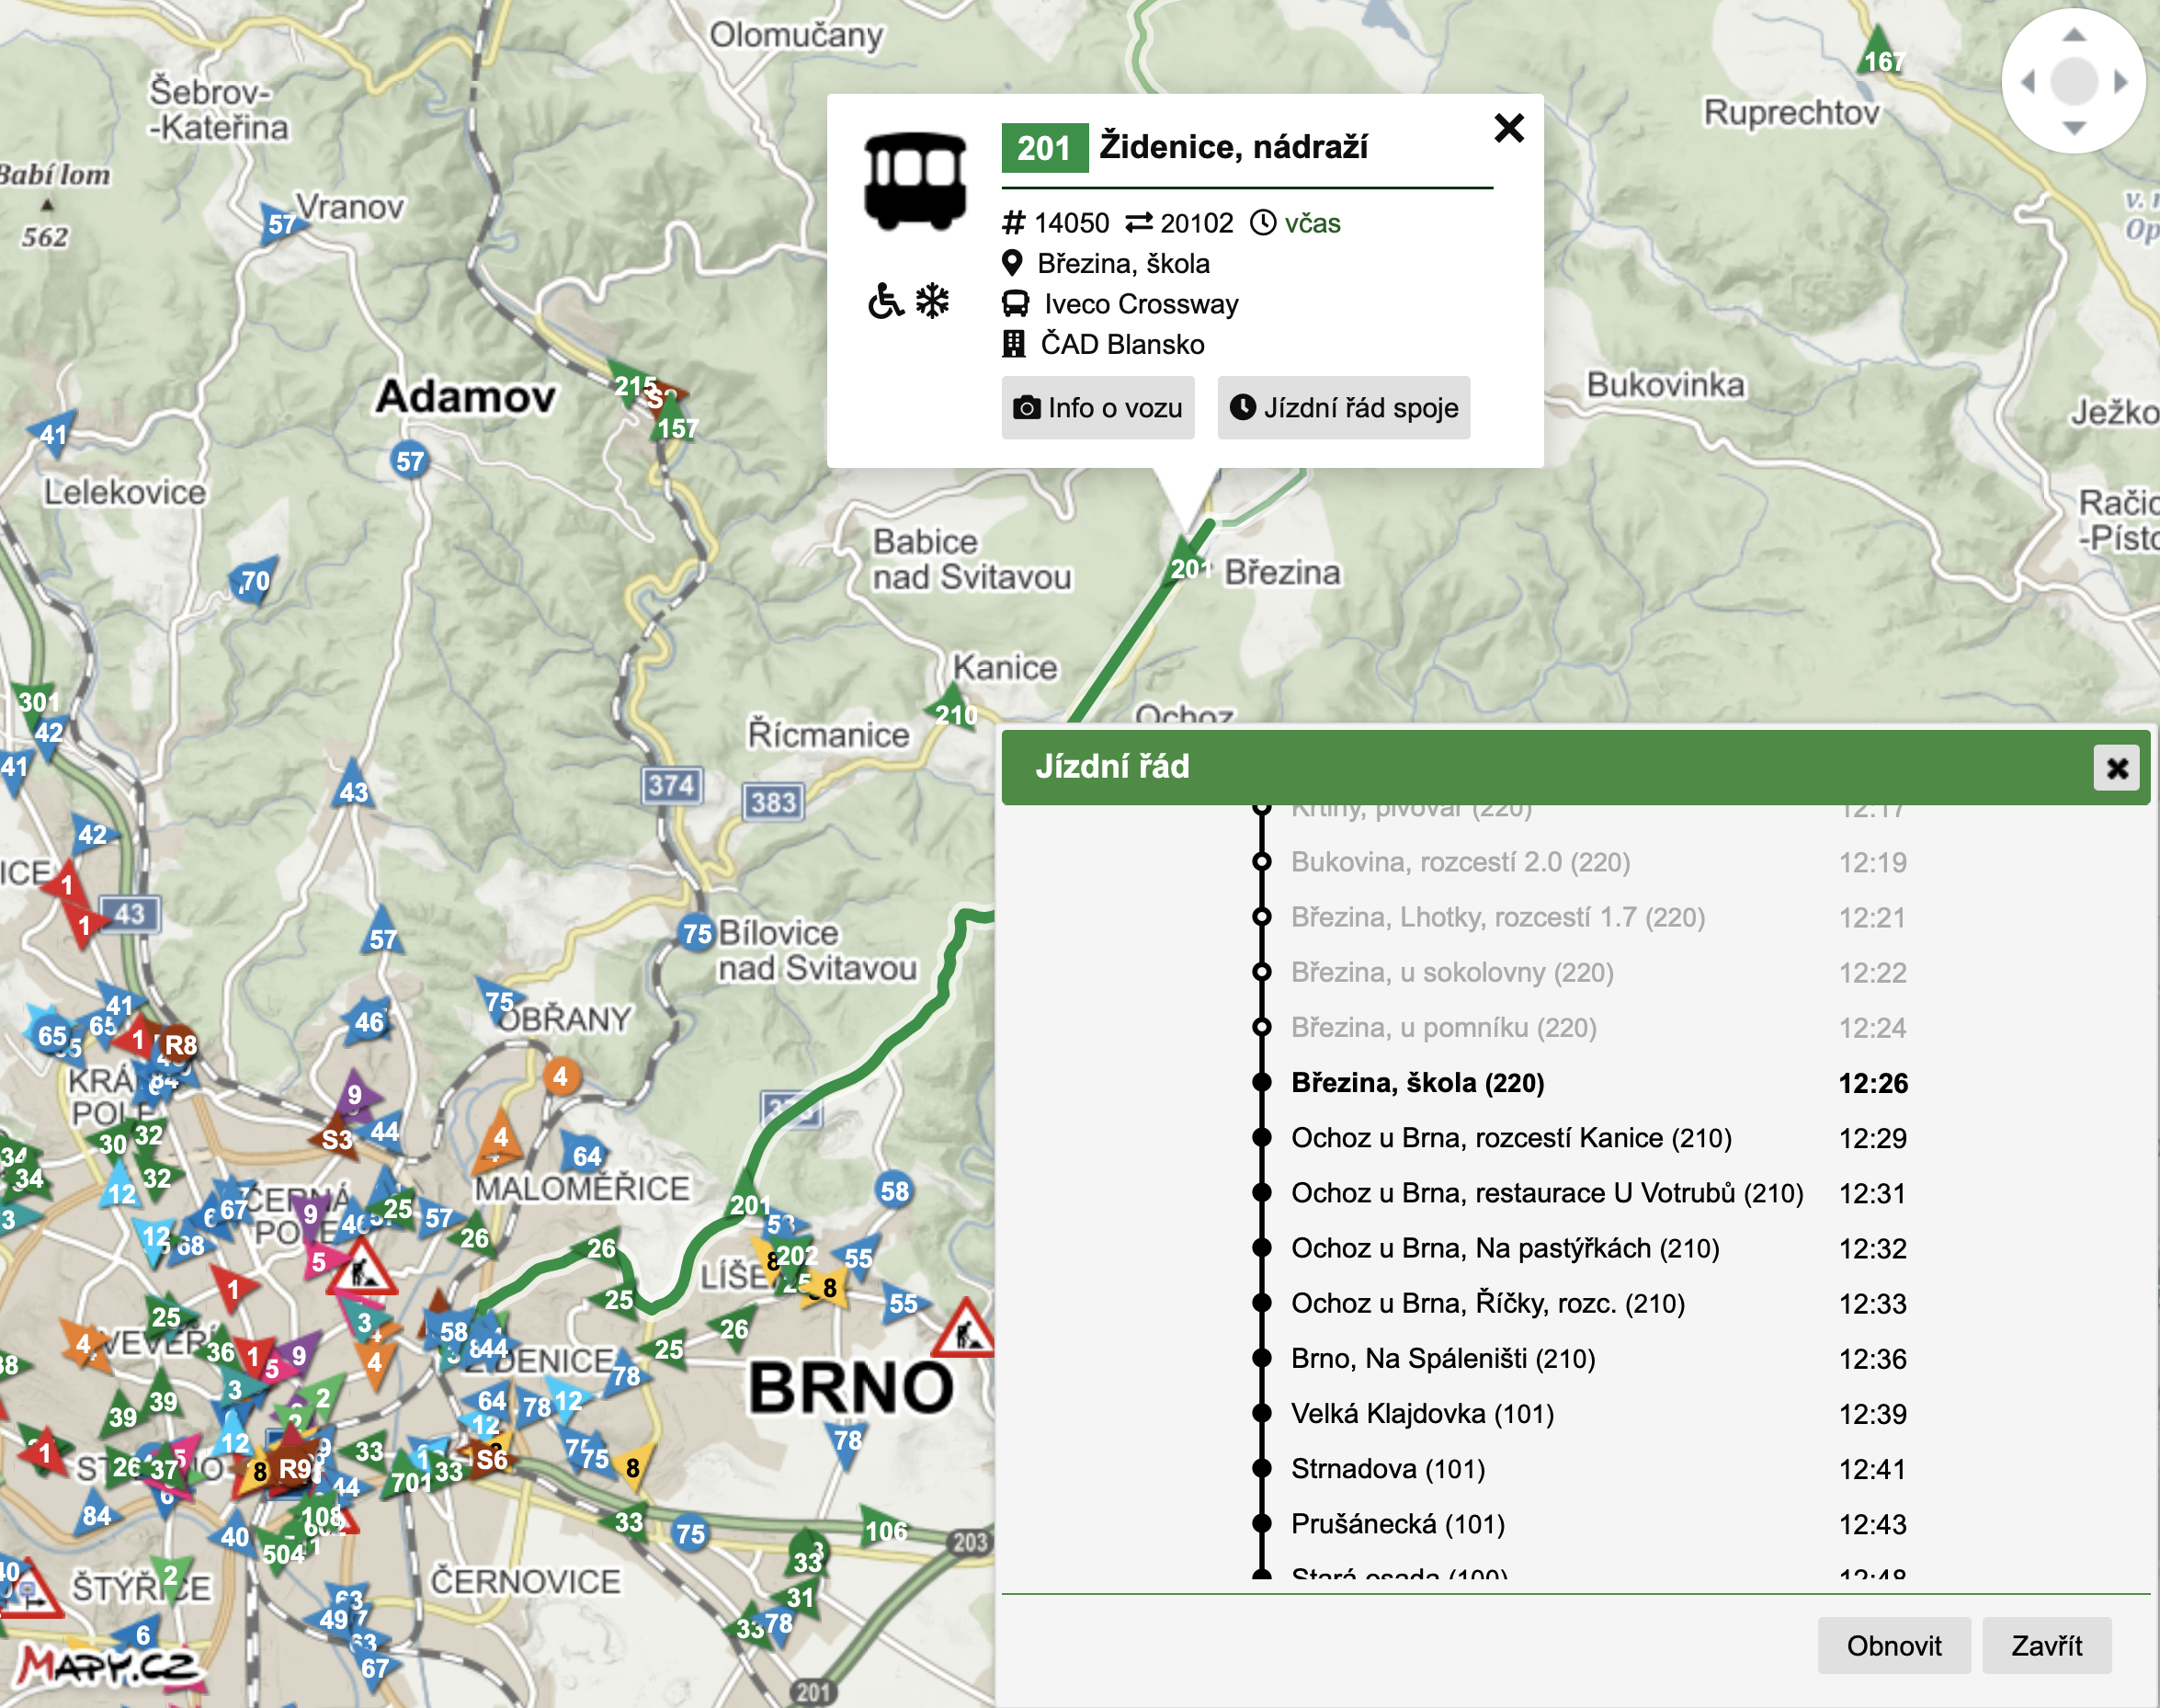
\includegraphics[width=\linewidth]{../img/idsjmk_mapa.png}
  \caption{Mapa z mapa.idsjmk.cz.}
  \label{fig:idsjmk_result}
\end{figure}
